\subsubsection{German Philosophy: Calibration Tests}

To help illustrate what exactly these methods are picking up when comparing two texts, we start by showing the range of similarity scores between pairs of Hegel's own texts (Table \ref{tab:hegelself}).

%Then, branching outwards, we compare a work of Hegel's with philosophical works from
%\begin{itemize}
%    \item[(a)] Two ``center'' Hegelians: Karl Ludwig Michelet and Karl Rosenkranz
%    \item[(b)] A ``Right Hegelian'', Johann Philipp Gabler, and
%    \item[(c)] two ``Left Hegelians'', Bruno Bauer and Ludwig Feuerbach (chosen to contrast someone Marx had a personal relationship with -- Bauer -- against someone with whom he only had a scholarly correpondence -- Feuerbach.)
%\end{itemize}

The results of the similarity tests among Hegel's own texts are given in Table \ref{tab:hegelself}. 

%and the results of the comparisons of Hegel with the subsequent Hegelians are given in Table \ref{tab:hegelians}.

\begin{table}[ht!]
\centering
\caption{Self-similarity between Hegel's works, using the embedding-based measure}
\label{tab:hegelself}
\begin{tabular}{lrrrr}
\toprule
{} &  Phänomenologie (1807) &  Geistes (1817) &  Logik (1817) &  Natur (1817) \\
\midrule
Phänomenologie (1807) &                 1.0000 &              -- &            -- &            -- \\
Geistes (1817)        &                 0.9635 &          1.0000 &            -- &            -- \\
Logik (1817)          &                 0.9478 &          0.9568 &        1.0000 &            -- \\
Natur (1817)          &                 0.8770 &          0.8653 &        0.8920 &        1.0000 \\
\bottomrule
\end{tabular}
\end{table}




\subsubsection{German Philosophy: Results}

A plot with Marx's semantic similarity to Hegel (by work, over time) can be found in Figure \ref{fig:hegelsims}, with the corresponding numeric similarity scores presented in Table \ref{tab:hegelsims}.

\begin{table}
\centering
\caption{Similarities between Marx and Hegel's works, over time}
\label{tab:hegelsim}
\begin{tabular}{lrrrrr}
\toprule
{} &  Phänomenologie (1807) &  Logik (1817) &  Natur (1817) &  Geistes (1817) &   Mean \\
\midrule
Differenz (1841)         &                 0.8612 &        0.8881 &        0.9136 &          0.8691 & 0.8830 \\
Zensor (1842)            &                 0.8288 &        0.8421 &        0.7868 &          0.8561 & 0.8284 \\
Hegel Critique (1843)    &                 0.8539 &        0.8588 &        0.8072 &          0.8814 & 0.8503 \\
Holy Family (1844)       &                 0.8427 &        0.8280 &        0.8426 &          0.8520 & 0.8413 \\
1844 Manus (1844)        &                 0.8521 &        0.8297 &        0.8107 &          0.8620 & 0.8386 \\
German Ideology (1846)   &                 0.8738 &        0.8621 &        0.8833 &          0.8894 & 0.8772 \\
Misere (1847)            &                 0.7692 &        0.7908 &        0.8088 &          0.7760 & 0.7862 \\
Manifesto (1848)         &                 0.6632 &        0.6163 &        0.6640 &          0.6500 & 0.6484 \\
18th Brumaire (1852)     &                 0.7092 &        0.6912 &        0.7549 &          0.7194 & 0.7186 \\
Grundrisse (1858)        &                 0.7191 &        0.7500 &        0.7727 &          0.7335 & 0.7438 \\
Kritik (1859)            &                 0.7169 &        0.7554 &        0.7971 &          0.7169 & 0.7466 \\
Herr Vogt (1860)         &                 0.6162 &        0.6446 &        0.7422 &          0.6546 & 0.6644 \\
Mehrwert 1 (1862)        &                 0.6066 &        0.6323 &        0.6540 &          0.6439 & 0.6342 \\
Mehrwert 2 (1862)        &                 0.5887 &        0.6382 &        0.6523 &          0.6341 & 0.6283 \\
Mehrwert 3 (1862)        &                 0.6263 &        0.6606 &        0.6718 &          0.6593 & 0.6545 \\
Lohn (1865)              &                 0.6673 &        0.7020 &        0.6958 &          0.6928 & 0.6895 \\
Kapital V1 (1867)        &                 0.6848 &        0.7039 &        0.7648 &          0.6975 & 0.7128 \\
Civ War in France (1871) &                 0.6798 &        0.6525 &        0.7321 &          0.6878 & 0.6880 \\
Gotha (1875)             &                 0.7111 &        0.7225 &        0.7099 &          0.7403 & 0.7210 \\
Kapital V2 (1885)        &                 0.5986 &        0.6251 &        0.6652 &          0.6136 & 0.6256 \\
Kapital V3 (1894)        &                 0.6258 &        0.6578 &        0.6861 &          0.6412 & 0.6527 \\
\bottomrule
\end{tabular}
\end{table}


\begin{figure}[ht!]
    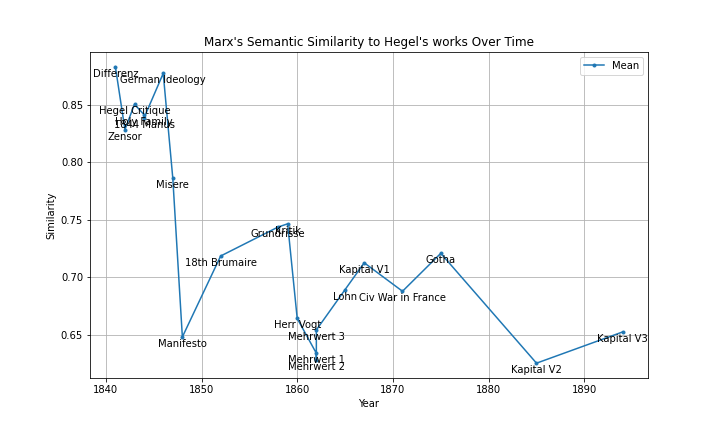
\includegraphics[width=\textwidth]{Emb0_Hegel_de_ts.png}
    \caption{Marx's similarity to Hegel, over time}
    \label{fig:hegelsims}
\end{figure}

Interestingly, given that many scholars locate Marx's departure from Hegel in his critical engagement with the latter's \textit{Philosophie des Rechts} in 1843, in terms of semantic content Marx's engagement with Hegelian \textit{themes} actually increases fairly dramatically after this time. This makes sense, however, if we consider the period roughly from 1843-1846 as a period wherein Marx aimed to distance himself from the Young Hegelians precisely by attacking their Hegel-oriented doctrines in the \textit{Holy Family} as well as the \textit{German Ideology}, and then the period from 1847 onward as his transition into his final economist phase. In fact, from what I can tell, the opening pages of the 1847 \textit{Misère de la Philosophie} are the first in which Marx explicitly identifies himself as an economist:

\begin{quote}
M. Proudhon has the misfortune to be uniquely misunderstood in Europe. In France he has the right to be a bad economist, since he passes for a good German philosopher. In Germany, he has the right to be a bad philosopher, because he passes as a prominent French economist. Being ourselves both German and economist, we have wished to protest against this dual mistake.\footnote{In Marx's original French: ``M. Proudhon a le malheur d'être singulièrement meconnu en Europe. En France, il a le droit d'être mauvais économiste, parce qu'il passe pour être bon philosophe allemand. En Allemagne, il a le droit d'être mauvais philosophe, parce qu'il passe pour être économiste français des plus forts. Nous, en notre qualité d'Allemand et d'économiste a la fois, nous avons voulu protester contre cette double erreur'' (\oldmega{I}{6}{19}; \textit{Misère} will also appear in its original French in the not-yet-published \mega{I}{6}).} (\mecw{6}{109}, as quoted in \cite{tribe_economy_2015})
\end{quote}


% Right after the German results

\subsubsection{French Republicanism: Calibration Tests}

To again establish our expectations with respect to what the similarity scores are capturing, we first show the similarity results for the set of Proudhon's texts included in our corpus.

%well-established relationships of direct influence:
%\begin{itemize}
%    \item[(a)] Saint-Simon vs. the ``Saint-Simonians''
%    \item[(b)] Babeuf vs. the ``Babeuvists'', and most importantly
%    \item[(c)] Proudhon vs. the ``Proudhonists''.
%\end{itemize}

These pairwise similarity scores between Proudhon's works are given in Table \ref{tab:proudhonself}.

\begin{table}[ht!]
\centering
\caption{Self-similarity between Proudhon's works, using the embedding-based measure}
\label{tab:proudhonself}
\begin{tabular}{lrrrr}
\toprule
{} &  Eigentum &  Nothwendigkeit &  Bekenntnisse &  Solution \\
\midrule
Eigentum       &    1.0000 &              -- &            -- &        -- \\
Nothwendigkeit &    0.9586 &          1.0000 &            -- &        -- \\
Bekenntnisse   &    0.9120 &          0.9316 &        1.0000 &        -- \\
Solution       &    0.9478 &          0.9529 &        0.8992 &    1.0000 \\
\bottomrule
\end{tabular}
\end{table}




\subsubsection{French Republicanism: Results}

Similarities between Marx's works and those of Proudhon are given in Figure \ref{fig:proudhonsims}, with the corresponding figures given in Table \ref{tab:proudhonsims}.

\begin{figure}
    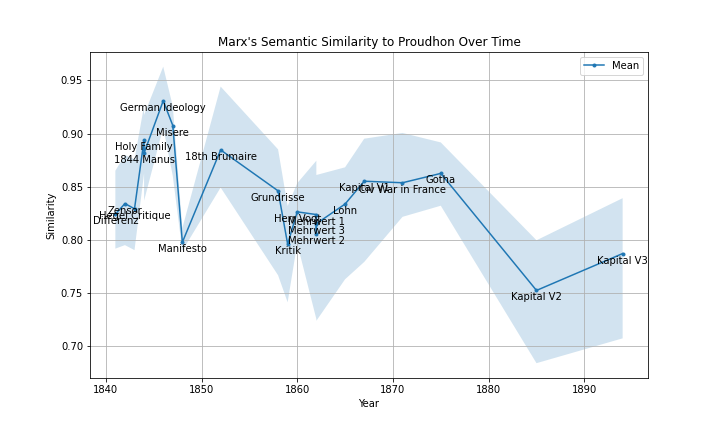
\includegraphics[width=\textwidth]{Emb1_Proudhon_de_ts.png}
    \caption{Marx's similarity to Proudhon, over time}
    \label{fig:proudhonsims}
\end{figure}

\begin{table}
\centering
\caption{Similarities between Marx's and Proudhon, over time}
\label{tab:proudhonsims}
\begin{tabular}{lrrrrr}
\toprule
{} &  Eigentum (1840) &  Nothwendigkeit (1847) &  Bekenntnisse (1848) &  Solution (1849) &   Mean \\
\midrule
Differenz (1841)         &           0.8072 &                 0.8651 &               0.8326 &           0.7919 & 0.8242 \\
Zensor (1842)            &           0.8231 &                 0.8389 &               0.8798 &           0.7952 & 0.8343 \\
Hegel Critique (1843)    &           0.8346 &                 0.8164 &               0.8759 &           0.7905 & 0.8294 \\
Holy Family (1844)       &           0.8733 &                 0.9263 &               0.9149 &           0.8627 & 0.8943 \\
1844 Manus (1844)        &           0.9176 &                 0.8992 &               0.8369 &           0.8733 & 0.8817 \\
German Ideology (1846)   &           0.9270 &                 0.9629 &               0.9277 &           0.9058 & 0.9308 \\
Misere (1847)            &           0.9188 &                 0.9257 &               0.8603 &           0.9257 & 0.9076 \\
Manifesto (1848)         &           0.7920 &                 0.8113 &               0.7899 &           0.7985 & 0.7979 \\
18th Brumaire (1852)     &           0.8493 &                 0.8711 &               0.9442 &           0.8740 & 0.8847 \\
Grundrisse (1858)        &           0.8749 &                 0.8579 &               0.7669 &           0.8852 & 0.8462 \\
Kritik (1859)            &           0.7980 &                 0.8132 &               0.7415 &           0.8320 & 0.7962 \\
Herr Vogt (1860)         &           0.7969 &                 0.8534 &               0.8274 &           0.8282 & 0.8265 \\
Mehrwert 1 (1862)        &           0.8746 &                 0.8370 &               0.7257 &           0.8585 & 0.8239 \\
Mehrwert 2 (1862)        &           0.8527 &                 0.8148 &               0.7152 &           0.8416 & 0.8061 \\
Mehrwert 3 (1862)        &           0.8611 &                 0.8243 &               0.7241 &           0.8520 & 0.8154 \\
Lohn (1865)              &           0.8683 &                 0.8456 &               0.7631 &           0.8581 & 0.8338 \\
Kapital V1 (1867)        &           0.8716 &                 0.8748 &               0.7794 &           0.8952 & 0.8553 \\
Civ War in France (1871) &           0.8218 &                 0.8537 &               0.9006 &           0.8392 & 0.8538 \\
Gotha (1875)             &           0.8917 &                 0.8645 &               0.8323 &           0.8619 & 0.8626 \\
Kapital V2 (1885)        &           0.7712 &                 0.7554 &               0.6843 &           0.7998 & 0.7526 \\
Kapital V3 (1894)        &           0.8119 &                 0.7903 &               0.7076 &           0.8393 & 0.7873 \\
\bottomrule
\end{tabular}
\end{table}



\subsubsection{British Political Economy: Calibration Tests}

As we did for German philosophy and French republican socialism, here we first examine the range of similarity measures our methods produce for a pair of books with an ``established'' relationship of influence: Adam Smith's \textit{Wealth of Nations} (1776) and David Ricardo's \textit{On the Principles of Political Economy and Taxation} (1817), given that the latter is in large part written as a response to Smith's groundbreaking 1776 work\footnote{Unlike in the previous two sections, here we opt not to compare Smith's \textit{Wealth of Nations} with e.g. his own earlier \textit{Theory of Moral Sentiments}, on the grounds that our aim is not to capture ``Smith-ness'' writ large, but rather ``political-economy-ness'' in the tradition established by \textit{Wealth of Nations}, rather than the less influential and more political-philosophy-oriented \textit{Theory of Moral Sentiments}. In Appendix \ref{app:robustness}, for transparency, we provide a version of Table \ref{tab:peself} which incorporates the \textit{Theory of Moral Sentiments} as well.}.

%set of ``established'' relationships of influence:
%\begin{itemize}
%    \item[(a)] Adam Ferguson vs. Adam Smith
%    \item[(b)] Adam Smith vs. David Ricardo, and
%    \item[(c)] John Stuart Mill's \textit{Principles} vs. David Ricardo's \textit{Political Economy}, of which the former work was explicitly written by Mill with the goal of ``formalizing'' the insights and contributions of the latter work.
%\end{itemize}

The results of these calibration tests are given in Table \ref{tab:peself}.

\begin{table}[ht!]
\centering
\caption{Self-similarity between Works of Political Economy, using the embedding-based measure}
\label{tab:peself}
\begin{tabular}{lrr}
\toprule
{} &  Wealth of Nations (2014) &  Grundgesetze (1877) \\
\midrule
Wealth of Nations (2014) &                    1.0000 &                   -- \\
Grundgesetze (1877)      &                    0.9400 &               1.0000 \\
\bottomrule
\end{tabular}
\end{table}



\subsubsection{British Political Economy: Results}

As can be seen in Figure \ref{fig:pesims} and Table \ref{tab:pesims}, Marx's ``Smith-ness'' increases significantly -- by over 10\% -- from his 1841 dissertation to his 1844 Manuscripts, then increases significantly but less rapidly in \textit{Poverty of Philosophy} and reaches a peak in 1858-1867 with the \grundrisse{}, the \kritik{}, the three volumes of \mehrwert{}, and \kapital{1}, with the notable exception of the extremely non-political-economic \textit{Herr Vogt}.

\begin{table}
\centering
\caption{Similarities between Marx's works and Works of Political Economy, over time}
\label{tab:pesims}
\begin{tabular}{lrrr}
\toprule
{} &  Grundgesetze (1838) &  Wealth of Nations (2014) &   Mean \\
\midrule
Differenz (1841)         &               0.7565 &                    0.7395 & 0.7480 \\
Zensor (1842)            &               0.7161 &                    0.7262 & 0.7211 \\
Hegel Critique (1843)    &               0.7289 &                    0.7224 & 0.7257 \\
Holy Family (1844)       &               0.7923 &                    0.7923 & 0.7923 \\
1844 Manus (1844)        &               0.8625 &                    0.8206 & 0.8416 \\
German Ideology (1846)   &               0.8606 &                    0.8441 & 0.8524 \\
Misere (1847)            &               0.9290 &                    0.9067 & 0.9178 \\
Manifesto (1848)         &               0.7718 &                    0.7709 & 0.7714 \\
18th Brumaire (1852)     &               0.7968 &                    0.7976 & 0.7972 \\
Grundrisse (1858)        &               0.9315 &                    0.8853 & 0.9084 \\
Kritik (1859)            &               0.8866 &                    0.8942 & 0.8904 \\
Herr Vogt (1860)         &               0.7584 &                    0.7286 & 0.7435 \\
Mehrwert 1 (1862)        &               0.9070 &                    0.8169 & 0.8620 \\
Mehrwert 2 (1862)        &               0.9174 &                    0.8133 & 0.8654 \\
Mehrwert 3 (1862)        &               0.9113 &                    0.8265 & 0.8689 \\
Lohn (1865)              &               0.9260 &                    0.8683 & 0.8971 \\
Kapital V1 (1867)        &               0.9314 &                    0.8985 & 0.9150 \\
Civ War in France (1871) &               0.7766 &                    0.7935 & 0.7850 \\
Gotha (1875)             &               0.8359 &                    0.7897 & 0.8128 \\
Kapital V2 (1885)        &               0.8654 &                    0.8077 & 0.8365 \\
Kapital V3 (1894)        &               0.9169 &                    0.8741 & 0.8955 \\
\bottomrule
\end{tabular}
\end{table}


\begin{figure}
    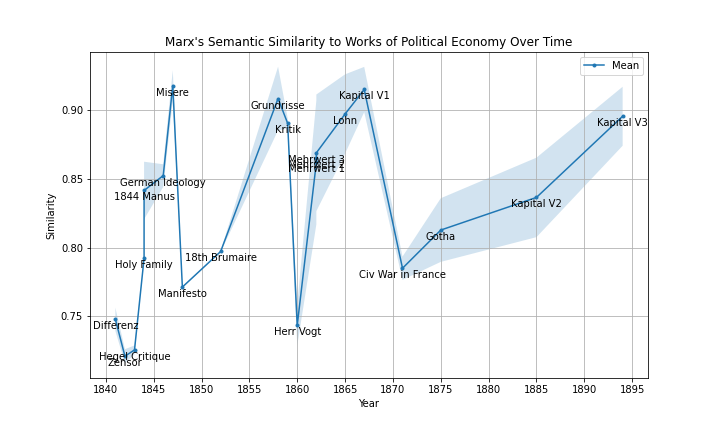
\includegraphics[width=\textwidth]{Emb2_PolEcon_de_ts.png}
    \caption{Marx's similarity to works of Political Economy, over time}
    \label{fig:pesims}
\end{figure}
